\documentclass[a4paper, 10pt]{article}
\usepackage[spanish] {babel}
\title{Taller 1}
\usepackage{caratula}
\usepackage[pdftex]{graphicx}
\usepackage{amssymb}

\setlength{\leftmargin}{2cm}
\setlength{\rightmargin}{2cm}
\setlength{\oddsidemargin}{-1cm}
\setlength{\evensidemargin}{-1cm}
\setlength{\topmargin}{-1cm}
\setlength{\textwidth}{18cm}
\setlength{\textheight}{25cm}


\usepackage{fancyhdr}
\pagestyle{fancy}
\fancyhf{}
\fancyhead [L]{\scriptsize Trabajo Pr\'actico N$^{\circ}$1}
\fancyhead [R]{\scriptsize Mancuso, Mataloni}%1{20pt}
\fancyfoot[C]{\thepage}
\renewcommand{\footrulewidth}{0.4pt}

\begin{document}
\materia{Sistemas Operativos}
\submateria{Primer Cuatrimestre de 2010}
\titulo{Taller N$^{\circ}$1}
\subtitulo{Schedulers}
\grupo{Grupo}
\integrante{Mataloni Alejandro}{706/07}{amataloni@gmail.com}
\integrante{Mancuso Emiliano}{597/07}{emiliano.mancuso@gmail.com}
\maketitle

\newpage

\section{Ejercicio 1}
  Partiendo de los 2 gr\'aficos de la c\'atedra identificamos los distintos tiempos de cada proceso. Identificamos 3 procesos y un tiempo IDLE del procesador, lo que nos dio el pie para averiguar a partir de que momento los procesos estaban listos. \newline
  Hasta ahora son 5 ciclos que el procesador esta en IDLE, el P1 demora 10 ciclos y P2 y P3 demoran 5 ciclos cada uno.
  Con el primer gr\'afico (FCFS) sabemos el orden de llegada de los procesos, que es justamente P1,P2,P3 y con el segundo (SJF) nos damos cuenta de que los tres procesos est\'an listos al mismo tiempo.\\

 \textbf{  Configuraci\'on de procesos}
  \begin{center}
  	\begin{tabular}{lll}
  		& Demora & Listo \\
  		P1 & 10 & 5 \\
  		P2 & 5 & 5 \\
  		P3 & 5 & 5 \\
  	\end{tabular}
  \end{center}



\section{Ejercicio 2}

  Para calcular el $waitingTime$ de cada tarea sin tener que modificar cada algoritmo, implementamos una funci\'on $finalize$ que adem\'as de dar por finalizada la tarea, calcula el tiempo de espera. \\

\begin{tabular}{rp{12cm}}
1: & public void finalize(int current\_time)\{\\
2: & \hspace{0,5cm} 	this.ftime = current\_time;\\
3: & \hspace{0,5cm} 	this.wtime = (ftime - rtime) - ptime;\\
4: & \}\\
 & \\ 
 & \texttt{ftime: finished time} \\
 & \texttt{rtime: ready time} \\
 & \texttt{ptime: process time} \\
\end{tabular}\\

\section{Ejercicio 3}
Gracias al dise\~no de la clase $Task$ que almacena el el tiempo de espera de cada tarea y a los algoritmos de Scheduling que conservan las tareas finalizadas, calcular el tiempo de espera promedio se resuelve con una sencilla cuenta.\\

\begin{tabular}{rp{12cm}}
1: & public double get\_avg\_wtime()\{\\
2: & \hspace{0,5cm} 	double avg = 0.0;\\
3: & \hspace{0,5cm} 	for (Task t : this.task\_set)\\
4: & \hspace{1,0cm} 	avg += t.wtime;\\
5: & \\
6: & \hspace{0,5cm} 	return avg / this.task\_set.size();\\
7: & \}\\
\end{tabular}\\

\newpage

\section{Ejercicio 4}
\begin{center}
	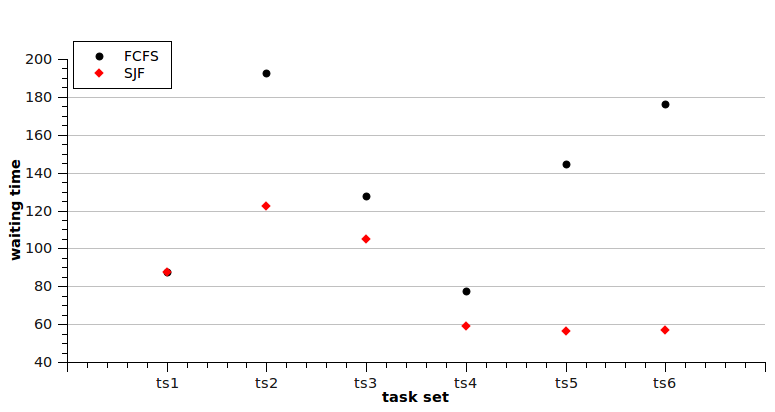
\includegraphics[scale=0.4]{graficos/waitingTime_FCFS-SJF.png}
\end{center}

 	Realizando el estudio utilizando los $taskset$ de la c\'atedra pudimos observar el comportamiento (en cuanto al waiting time de los procesos) de los schedulers del tipo $FCFS$ y $SJF$. El waiting time promedio es menor en $SJF$. Esto se debe a que justamente con \'esta pol\'itica garantiza que los que menos tardan se ejecutan primero y de esta manera se evita que un proceso que tarda mucho le sume waiting time a otros procesos mas cortos.
 

\section{Ejercicio 5}
	Realizando varios estudios sobre el comportamiento de $RR$ utilizando diferentes quantums observamos que a medida que se le asigna un mayor valor, el tiempo de espera promedio disminuye. Esto se debe a que los procesos en un quantum asignado pueden ejecutar m\'as, por lo tanto van a terminar m\'as r\'apido. Es decir, mientras m\'as interrupciones tenga un proceso, crece el tiempo de espera promedio. Para obtener un mejor promedio se aumenta el valor del quantum pero verificando que no se perjudiquen los beneficios del algoritmo de scheduler.

Si el quantum toma el m\'aximo tiempo de proceso, de alg\'un proceso en el taskset, se pierde el preemption que ofrece el algoritmo.
Por eso, nosotros encontramos como buen valor el promedio de los tiempos de proceso dentro de un mismo TaskSet, para disminuir el tiempo de espera promedio.

\begin{center}
	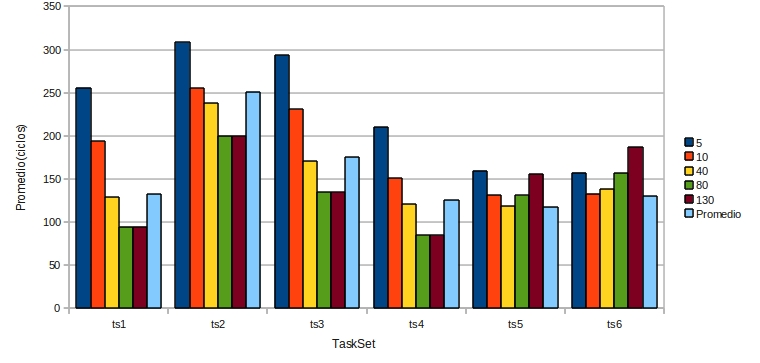
\includegraphics[scale=0.4]{graficos/ejercicio5_RR.jpg}
\end{center}

\begin{center}
	\begin{tabular}{|r|r|r|r|r|r|r|}
	  \hline
		    &  5 & 10 & 40 & 80 & 130 & Promedio \\
	  \hline
		ts1 & 255.75 & 193.5 & 128.5 & 94.5 & 94.5 & 132.25 \\
	  \hline
		ts2 & 308.25 & 255 & 237.5 & 199.5 & 199.5 & 251.25 \\
		\hline
		ts3 & 293.375 & 230.5 & 170.25 & 134.5 & 134.5 & 175.25 \\
		\hline
		ts4 & 210.125 & 150.5 & 120.25 & 84.5 & 84.5 & 125.25 \\
		\hline
		ts5 & 159.625 & 131.125 & 118.125 & 130.75 & 155.75 & 117.325 \\
		\hline
		ts6 & 157.3 & 132.8 & 138.7 & 156.9 & 186.9 & 130.1 \\
		\hline
	\end{tabular}
	\label{tab:}
\end{center}

Como se puede ver el en gr\'afico, para los primeros TaskSet el quantum de tama\~no promedio es de los que mantienen el menor Waiting Time.


\newpage
\section{Ejercicio 6}
	 En el caso de Multilevel Feedback Queue, es un algoritmo m\'as complejo que los anteriores y se podr\'ia ubicar entre los algoritmos de $SJF$ y $RR$.
	
Para comparar los algoritmos de scheduling, los comparamos analizando el turnaround promedio.\\

\begin{center}
	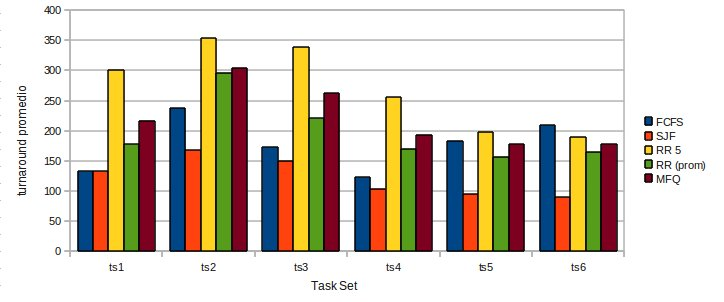
\includegraphics[scale=0.6]{graficos/turnArround.jpg}
\end{center}
En el gr\'afico podemos observar que el algoritmo MFQ se comporta muy parecido al RR, esto se debe al preemption que define la especificaci\'on de la c\'atedra. \\


Lo que queremos decir es que, para optimizar el turnaround los procesos m\'as cortos est\'an en las colas con m\'as prioridad, mientras que los m\'as largos van disminuyendo su prioridad a trav\'es de las colas.\\
 A su vez, para no comportarse como un $SJF$ se introducen las colas y el preemption y ahi es donde se acerca a la idea de un $RR$. Con \'esta optimiza el tiempo de respuesta en el sistema, beneficiando los procesos interactivos y reduciendo la probabilidad de que un proceso caiga en inanici\'on en comparaci\'on con $SJF$, sin embargo, no elimina por completo la inanici\'on.\\

Supongamos el caso en que existe un proceso que requiere un largo tiempo de ejecuci\'on y junto con el, muchos procesos con un tiempo de ejecuci\'on suficiente para ser atendidos en la cola de alta prioridad.
El proceso m\'as largo se ejecuta al principio, cuando permanece en la cola de alta prioridad y va descendiendo por las diferentes colas. Al mismo tiempo nuevos procesos ingresan en la cola de alta prioridad, haciendo que el proceso largo no sea atendido y caiga en inanici\'on mientras los procesos en la cola de alta prioridad entran y se ejecutan.\\

La mayor\'ia de los procesos interactivos, son procesos largos pero requieren ser atendidos de inmediato, por lo tanto para no caer en inanici\'on estos procesos son 'premiados' cuando hacen E/S (en el algoritmo de MFQ con IO).

\end{document}

